\documentclass{standalone}
\usepackage{libertinus}
\usepackage{tikz}
\usetikzlibrary{matrix, patterns, backgrounds, positioning}
\begin{document}
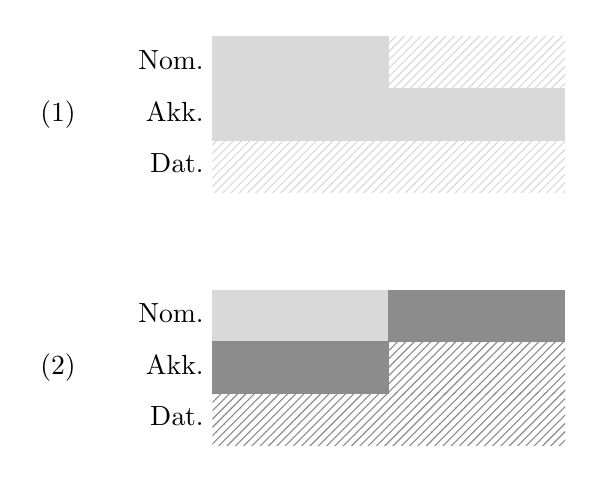
\begin{tikzpicture}
		\matrix [matrix of nodes,
		nodes in empty cells,
		align=right,
		nodes={text width=2cm, minimum height=1em, font=\strut}]
		(karpfen1)
		{
			Nom.& & \\
			Akk.& & \\
			Dat.& & \\
		};
		\fill [fill=gray!30] 
		(karpfen1-1-2.north west) rectangle (karpfen1-2-2.south east);
		\fill [fill=gray!30]
		(karpfen1-2-3.north west) rectangle (karpfen1-2-3.south east);
		\fill [pattern=north east lines, pattern color=gray!30]
		(karpfen1-1-3.north west) rectangle (karpfen1-1-3.south east);
		\fill[pattern=north east lines, pattern color=gray!30]
		(karpfen1-3-2.north west) rectangle (karpfen1-3-3.south east);
		\node[left = 0.5cm of karpfen1-2-1.center] {(1)};

	\matrix [matrix of nodes,
	nodes in empty cells,
	align=right,
	below = of karpfen1,
	nodes={text width=2cm, minimum height=1em, font=\strut}]
	(karpfen2)
	{
		Nom.& & \\
		Akk.& & \\
		Dat.& & \\
	};
	\fill [fill=gray!30] 
	(karpfen2-1-2.north west) rectangle (karpfen2-1-2.south east);
	\fill [fill=gray!90]
	(karpfen2-1-3.north west) rectangle (karpfen2-1-3.south east);
	\fill[gray!90]
	(karpfen2-2-2.north west) rectangle (karpfen2-2-2.south east);
	\fill [pattern=north east lines, pattern color=gray!90]
	(karpfen2-2-3.north west) rectangle (karpfen2-2-3.south east);
	\fill [pattern=north east lines, pattern color=gray!90]
	(karpfen2-3-2.north west) rectangle (karpfen2-3-3.south east);
	\node[left = 0.5cm of karpfen2-2-1.center] {(2)};
\end{tikzpicture}
\end{document}